\documentclass{book}
\usepackage[landscape,a3paper,left=0.5cm,right=1in,top=1in,bottom=1in]{geometry}
\usepackage{amsmath}
\usepackage{xcolor}
\usepackage{tikz}
\usepackage{pgfplots}
\usepackage{booktabs}
\usepackage{multirow}
\usepackage{amsmath,amssymb}

\begin{document}

\vspace{2cm}

\begin{center}\underline{\textsc{Equiv + Permut} for Test of 99 small instances of knapsack}
\vspace{0.5cm}

\begin{tabular}{ccc} & cp-sat & chuffed\\\\\tikz{\node (a) at (0.0,4) {\textsc{QuadraMod}};\node (a) at (0.0,0) {};} & 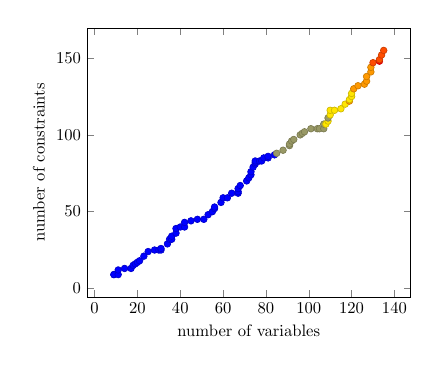
\begin{tikzpicture}[scale=0.6]
\begin{axis}[scatter, point meta=\thisrow{time}, only marks, colorbar, colorbar horizontal,colorbar style={ylabel={Time (min)}, ylabel style={rotate=270},}, colorbar to name={storedcolorbar1},, xlabel=number of variables,ylabel=number of constraints]

\addplot table[x=x,y=y]  { 
 x y time
 9 9 0.05 
 9 9 0.0 
 11 9 0.0 
 11 12 0.0 
 14 13 0.0 
 17 13 0.0 
 18 15 0.0 
 19 16 0.0 
 20 17 0.0 
 21 18 0.0 
 23 21 0.0 
 25 24 0.0 
 28 25 0.0 
 30 25 0.0 
 31 25 0.0 
 31 26 0.0 
 34 29 0.0 
 35 32 0.0 
 36 32 0.0 
 36 34 0.0 
 38 36 0.0 
 38 39 0.0 
 40 40 0.0 
 42 40 0.0 
 42 43 0.0 
 45 44 0.0 
 48 45 0.0 
 51 45 0.0 
 53 48 0.0 
 55 50 0.0 
 56 52 0.0 
 56 53 0.0 
 59 56 0.0 
 60 59 0.0 
 62 59 0.0 
 64 62 0.0 
 67 62 0.0 
 67 63 0.0 
 67 65 0.0 
 68 67 0.0 
 71 70 0.0 
 72 72 0.0 
 73 74 0.0 
 73 76 0.0 
 74 79 0.0 
 75 81 0.0 
 75 82 0.0 
 75 83 0.0 
 77 83 0.0 
 78 83 0.0 
 79 85 0.0 
 81 85 0.0 
 81 86 0.0 
 84 87 0.0 
 85 88 1.0 
 88 90 1.0 
 91 93 1.0 
 91 94 1.0 
 92 96 1.0 
 93 97 1.0 
 96 100 1.0 
 97 101 1.0 
 98 102 1.0 
 101 104 1.0 
 104 104 1.0 
 105 104 1.0 
 107 104 1.0 
 107 107 1.0 
 108 107 2.0 
 109 109 2.0 
 109 111 1.0 
 110 113 2.0 
 110 116 2.0 
 112 116 2.0 
 115 117 2.0 
 117 120 2.0 
 119 122 3.0 
 119 123 2.0 
 120 125 2.0 
 120 127 2.0 
 121 130 3.0 
 123 132 3.0 
 126 133 3.0 
 127 135 3.0 
 127 138 3.0 
 129 141 3.0 
 129 144 3.0 
 130 147 4.0 
 133 148 5.0 
 133 149 4.0 
 134 152 4.0 
 135 155 4.0 
};

\end{axis}
\end{tikzpicture}

 & 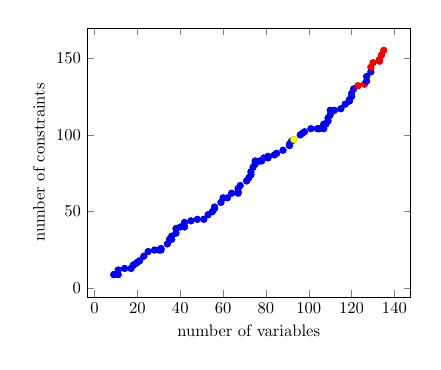
\begin{tikzpicture}[scale=0.6]
\begin{axis}[scatter, point meta=\thisrow{time}, only marks, , xlabel=number of variables,ylabel=number of constraints]

\addplot table[x=x,y=y]  { 
 x y time
 9 9 0.05 
 9 9 0.0 
 11 9 0.0 
 11 12 0.0 
 14 13 0.0 
 17 13 0.0 
 18 15 0.0 
 19 16 0.0 
 20 17 0.0 
 21 18 0.0 
 23 21 0.0 
 25 24 0.0 
 28 25 0.0 
 30 25 0.0 
 31 25 0.0 
 31 26 0.0 
 34 29 0.0 
 35 32 0.0 
 36 32 0.0 
 36 34 0.0 
 38 36 0.0 
 38 39 0.0 
 40 40 0.0 
 42 40 0.0 
 42 43 0.0 
 45 44 0.0 
 48 45 0.0 
 51 45 0.0 
 53 48 1.0 
 55 50 0.0 
 56 52 0.0 
 56 53 1.0 
 59 56 1.0 
 60 59 2.0 
 62 59 1.0 
 64 62 1.0 
 67 62 2.0 
 67 63 4.0 
 67 65 1.5 
 68 67 1.0 
 71 70 4.0 
 72 72 4.0 
 73 74 1.0 
 73 76 4.0 
 74 79 3.0 
 75 81 5.0 
 75 82 2.0 
 75 83 2.0 
 77 83 2.0 
 78 83 6.0 
 79 85 39.0 
 81 85 3.0 
 81 86 3.0 
 84 87 3.0 
 85 88 2.0 
 88 90 2.0 
 91 93 3.0 
 91 94 5.0 
 92 96 31.5 
 93 97 482.33 
 96 100 4.0 
 97 101 4.0 
 98 102 3.0 
 101 104 4.0 
 104 104 6.0 
 105 104 5.0 
 107 104 5.5 
 107 107 4.0 
 108 107 5.0 
 109 109 5.0 
 109 111 11.0 
 110 113 9.0 
 110 116 8.0 
 112 116 15.0 
 115 117 7.0 
 117 120 9.0 
 119 122 10.0 
 119 123 16.0 
 120 125 8.0 
 120 127 23.0 
 121 130 25.0 
 123 132 1440.0 
 126 133 1440.0 
 127 135 15.0 
 127 138 14.0 
 129 141 11.0 
 129 144 1440.0 
 130 147 1440.0 
 133 148 1440.0 
 133 149 1440.0 
 134 152 1440.0 
 135 155 1440.0 
};

\end{axis}
\end{tikzpicture}

\\
\tikz{\node (a) at (0.0,4) {\textsc{TheoMod}};\node (a) at (0.0,0) {};} & 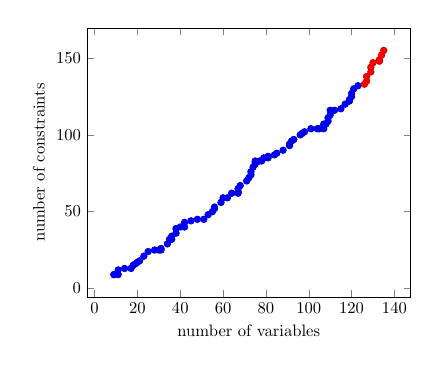
\begin{tikzpicture}[scale=0.6]
\begin{axis}[scatter, point meta=\thisrow{time}, only marks, , xlabel=number of variables,ylabel=number of constraints]

\addplot table[x=x,y=y]  { 
 x y time
 9 9 0.05 
 9 9 0.0 
 11 9 0.0 
 11 12 0.0 
 14 13 0.0 
 17 13 0.0 
 18 15 0.0 
 19 16 0.0 
 20 17 0.0 
 21 18 0.0 
 23 21 0.0 
 25 24 0.0 
 28 25 0.0 
 30 25 0.0 
 31 25 0.0 
 31 26 0.0 
 34 29 0.0 
 35 32 0.0 
 36 32 0.0 
 36 34 0.0 
 38 36 0.0 
 38 39 0.0 
 40 40 0.0 
 42 40 0.0 
 42 43 0.0 
 45 44 0.0 
 48 45 0.0 
 51 45 0.0 
 53 48 0.0 
 55 50 0.0 
 56 52 0.0 
 56 53 0.0 
 59 56 0.0 
 60 59 0.0 
 62 59 0.0 
 64 62 0.0 
 67 62 0.0 
 67 63 0.0 
 67 65 0.0 
 68 67 0.0 
 71 70 0.0 
 72 72 0.0 
 73 74 0.0 
 73 76 0.0 
 74 79 0.0 
 75 81 0.0 
 75 82 0.0 
 75 83 0.0 
 77 83 0.0 
 78 83 0.0 
 79 85 0.0 
 81 85 0.0 
 81 86 0.0 
 84 87 0.0 
 85 88 0.0 
 88 90 0.0 
 91 93 0.0 
 91 94 0.0 
 92 96 0.5 
 93 97 0.0 
 96 100 1.0 
 97 101 1.0 
 98 102 1.0 
 101 104 1.0 
 104 104 1.0 
 105 104 1.0 
 107 104 1.0 
 107 107 1.0 
 108 107 1.5 
 109 109 1.0 
 109 111 2.0 
 110 113 2.0 
 110 116 2.0 
 112 116 2.0 
 115 117 2.0 
 117 120 2.0 
 119 122 3.0 
 119 123 3.0 
 120 125 3.0 
 120 127 2.0 
 121 130 4.0 
 123 132 3.0 
 126 133 1440.0 
 127 135 1440.0 
 127 138 1440.0 
 129 141 1440.0 
 129 144 1440.0 
 130 147 1440.0 
 133 148 1440.0 
 133 149 1440.0 
 134 152 1440.0 
 135 155 1440.0 
};

\end{axis}
\end{tikzpicture}

 & 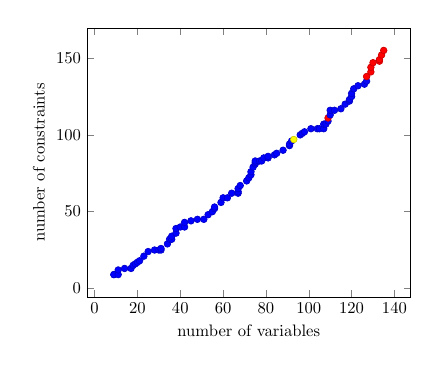
\begin{tikzpicture}[scale=0.6]
\begin{axis}[scatter, point meta=\thisrow{time}, only marks, , xlabel=number of variables,ylabel=number of constraints]

\addplot table[x=x,y=y]  { 
 x y time
 9 9 0.05 
 9 9 0.0 
 11 9 0.0 
 11 12 0.0 
 14 13 0.0 
 17 13 0.0 
 18 15 0.0 
 19 16 0.0 
 20 17 0.0 
 21 18 0.0 
 23 21 0.0 
 25 24 0.0 
 28 25 0.0 
 30 25 0.0 
 31 25 0.0 
 31 26 0.0 
 34 29 0.0 
 35 32 0.0 
 36 32 0.0 
 36 34 0.0 
 38 36 0.0 
 38 39 0.0 
 40 40 0.0 
 42 40 0.0 
 42 43 0.0 
 45 44 0.0 
 48 45 0.0 
 51 45 0.0 
 53 48 0.0 
 55 50 0.0 
 56 52 0.0 
 56 53 0.0 
 59 56 0.0 
 60 59 0.0 
 62 59 0.0 
 64 62 0.0 
 67 62 1.0 
 67 63 0.0 
 67 65 1.0 
 68 67 0.0 
 71 70 1.0 
 72 72 1.0 
 73 74 1.0 
 73 76 0.0 
 74 79 0.0 
 75 81 1.0 
 75 82 1.0 
 75 83 1.0 
 77 83 1.0 
 78 83 1.0 
 79 85 2.0 
 81 85 1.0 
 81 86 1.0 
 84 87 1.0 
 85 88 1.0 
 88 90 2.0 
 91 93 2.0 
 91 94 4.0 
 92 96 3.5 
 93 97 482.33 
 96 100 2.0 
 97 101 3.0 
 98 102 3.0 
 101 104 9.0 
 104 104 3.0 
 105 104 3.0 
 107 104 4.5 
 107 107 5.0 
 108 107 5.0 
 109 109 4.0 
 109 111 1440.0 
 110 113 5.0 
 110 116 5.0 
 112 116 6.0 
 115 117 7.0 
 117 120 8.0 
 119 122 7.0 
 119 123 8.0 
 120 125 9.0 
 120 127 8.0 
 121 130 9.0 
 123 132 9.0 
 126 133 11.0 
 127 135 16.0 
 127 138 1440.0 
 129 141 1440.0 
 129 144 1440.0 
 130 147 1440.0 
 133 148 1440.0 
 133 149 1440.0 
 134 152 1440.0 
 135 155 1440.0 
};

\end{axis}
\end{tikzpicture}

\\
\\\\
\multicolumn{3}{c}{\ref{storedcolorbar1}}\end{tabular}\end{center}

\newpage

\begin{center}\underline{\textsc{Non-Equiv + Permut} for Test of 99 small instances of knapsack}
\vspace{0.5cm}

\begin{tabular}{ccc} & cp-sat & chuffed\\\\\tikz{\node (a) at (0.0,4) {\textsc{QuadraMod}};\node (a) at (0.0,0) {};} & 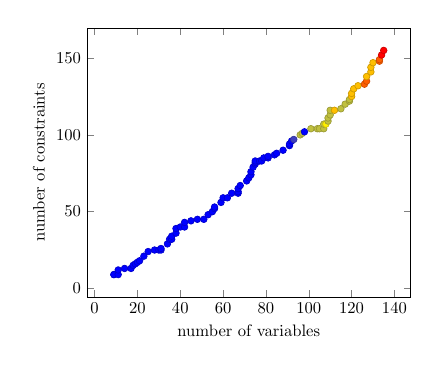
\begin{tikzpicture}[scale=0.6]
\begin{axis}[scatter, point meta=\thisrow{time}, only marks, colorbar, colorbar horizontal,colorbar style={ylabel={Time (min)}, ylabel style={rotate=270},}, colorbar to name={storedcolorbar2},, xlabel=number of variables,ylabel=number of constraints]

\addplot table[x=x,y=y]  { 
 x y time
 9 9 0.05 
 9 9 0.0 
 11 9 0.0 
 11 12 0.0 
 14 13 0.0 
 17 13 0.0 
 18 15 0.0 
 19 16 0.0 
 20 17 0.0 
 21 18 0.0 
 23 21 0.0 
 25 24 0.0 
 28 25 0.0 
 30 25 0.0 
 31 25 0.0 
 31 26 0.0 
 34 29 0.0 
 35 32 0.0 
 36 32 0.0 
 36 34 0.0 
 38 36 0.0 
 38 39 0.0 
 40 40 0.0 
 42 40 0.0 
 42 43 0.0 
 45 44 0.0 
 48 45 0.0 
 51 45 0.0 
 53 48 0.0 
 55 50 0.0 
 56 52 0.0 
 56 53 0.0 
 59 56 0.0 
 60 59 0.0 
 62 59 0.0 
 64 62 0.0 
 67 62 0.0 
 67 63 0.0 
 67 65 0.0 
 68 67 0.0 
 71 70 0.0 
 72 72 0.0 
 73 74 0.0 
 73 76 0.0 
 74 79 0.0 
 75 81 0.0 
 75 82 0.0 
 75 83 0.0 
 77 83 0.0 
 78 83 0.0 
 79 85 0.0 
 81 85 0.0 
 81 86 0.0 
 84 87 0.0 
 85 88 0.0 
 88 90 0.0 
 91 93 0.0 
 91 94 0.0 
 92 96 0.0 
 93 97 0.33 
 96 100 1.0 
 97 101 1.0 
 98 102 0.0 
 101 104 1.0 
 104 104 1.0 
 105 104 1.0 
 107 104 1.0 
 107 107 1.0 
 108 107 1.5 
 109 109 1.0 
 109 111 1.0 
 110 113 1.0 
 110 116 1.0 
 112 116 2.0 
 115 117 1.0 
 117 120 1.0 
 119 122 1.0 
 119 123 1.0 
 120 125 2.0 
 120 127 2.0 
 121 130 2.0 
 123 132 2.0 
 126 133 3.0 
 127 135 3.0 
 127 138 2.0 
 129 141 2.0 
 129 144 2.0 
 130 147 2.0 
 133 148 3.0 
 133 149 3.0 
 134 152 4.0 
 135 155 4.0 
};

\end{axis}
\end{tikzpicture}

 & 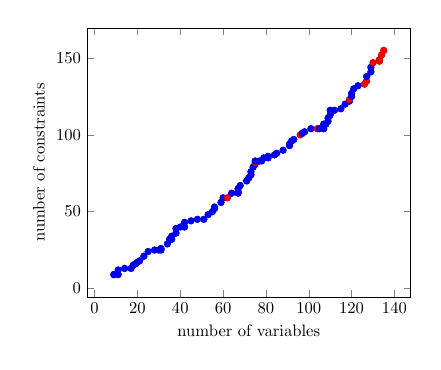
\begin{tikzpicture}[scale=0.6]
\begin{axis}[scatter, point meta=\thisrow{time}, only marks, , xlabel=number of variables,ylabel=number of constraints]

\addplot table[x=x,y=y]  { 
 x y time
 9 9 0.05 
 9 9 0.0 
 11 9 0.0 
 11 12 0.0 
 14 13 0.0 
 17 13 0.0 
 18 15 0.0 
 19 16 0.0 
 20 17 0.0 
 21 18 0.0 
 23 21 0.0 
 25 24 0.0 
 28 25 0.0 
 30 25 0.0 
 31 25 0.0 
 31 26 0.0 
 34 29 0.0 
 35 32 0.0 
 36 32 0.0 
 36 34 0.0 
 38 36 0.0 
 38 39 0.0 
 40 40 0.0 
 42 40 0.0 
 42 43 0.0 
 45 44 0.0 
 48 45 0.0 
 51 45 0.0 
 53 48 0.0 
 55 50 0.0 
 56 52 0.0 
 56 53 0.0 
 59 56 0.0 
 60 59 0.0 
 62 59 1440.0 
 64 62 0.0 
 67 62 1.0 
 67 63 1.0 
 67 65 1.0 
 68 67 1.0 
 71 70 1.0 
 72 72 1.0 
 73 74 1.0 
 73 76 1.0 
 74 79 1.0 
 75 81 2.0 
 75 82 1440.0 
 75 83 2.0 
 77 83 2.0 
 78 83 2.0 
 79 85 2.0 
 81 85 3.0 
 81 86 3.0 
 84 87 3.0 
 85 88 3.0 
 88 90 3.0 
 91 93 3.0 
 91 94 2.0 
 92 96 3.0 
 93 97 3.0 
 96 100 1440.0 
 97 101 3.0 
 98 102 3.0 
 101 104 4.0 
 104 104 1440.0 
 105 104 3.0 
 107 104 3.5 
 107 107 3.0 
 108 107 4.5 
 109 109 6.0 
 109 111 4.0 
 110 113 6.0 
 110 116 4.0 
 112 116 5.0 
 115 117 5.0 
 117 120 6.0 
 119 122 6.0 
 119 123 1440.0 
 120 125 6.0 
 120 127 7.0 
 121 130 6.0 
 123 132 8.0 
 126 133 1440.0 
 127 135 1440.0 
 127 138 8.0 
 129 141 10.0 
 129 144 11.0 
 130 147 1440.0 
 133 148 1440.0 
 133 149 1440.0 
 134 152 1440.0 
 135 155 1440.0 
};

\end{axis}
\end{tikzpicture}

\\
\tikz{\node (a) at (0.0,4) {\textsc{TheoMod}};\node (a) at (0.0,0) {};} & 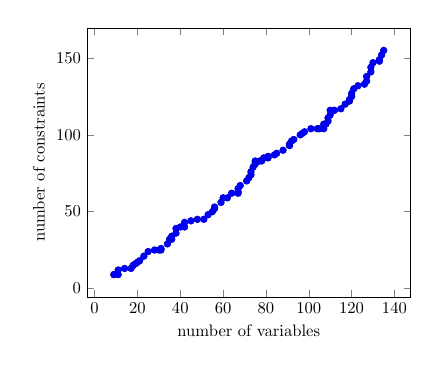
\begin{tikzpicture}[scale=0.6]
\begin{axis}[scatter, point meta=\thisrow{time}, only marks, , xlabel=number of variables,ylabel=number of constraints]

\addplot table[x=x,y=y]  { 
 x y time
 9 9 0.05 
 9 9 0.0 
 11 9 0.0 
 11 12 0.0 
 14 13 0.0 
 17 13 0.0 
 18 15 0.0 
 19 16 0.0 
 20 17 0.0 
 21 18 0.0 
 23 21 0.0 
 25 24 0.0 
 28 25 0.0 
 30 25 0.0 
 31 25 0.0 
 31 26 0.0 
 34 29 0.0 
 35 32 0.0 
 36 32 0.0 
 36 34 0.0 
 38 36 0.0 
 38 39 0.0 
 40 40 0.0 
 42 40 0.0 
 42 43 0.0 
 45 44 0.0 
 48 45 0.0 
 51 45 0.0 
 53 48 0.0 
 55 50 0.0 
 56 52 0.0 
 56 53 0.0 
 59 56 0.0 
 60 59 0.0 
 62 59 0.0 
 64 62 0.0 
 67 62 0.0 
 67 63 0.0 
 67 65 0.0 
 68 67 0.0 
 71 70 0.0 
 72 72 0.0 
 73 74 0.0 
 73 76 0.0 
 74 79 0.0 
 75 81 0.0 
 75 82 0.0 
 75 83 0.0 
 77 83 0.0 
 78 83 0.0 
 79 85 0.0 
 81 85 0.0 
 81 86 0.0 
 84 87 0.0 
 85 88 0.0 
 88 90 0.0 
 91 93 0.0 
 91 94 0.0 
 92 96 0.0 
 93 97 0.0 
 96 100 0.0 
 97 101 0.0 
 98 102 0.0 
 101 104 0.0 
 104 104 0.0 
 105 104 0.0 
 107 104 0.0 
 107 107 0.0 
 108 107 0.0 
 109 109 0.0 
 109 111 0.0 
 110 113 0.0 
 110 116 0.0 
 112 116 0.0 
 115 117 0.0 
 117 120 0.0 
 119 122 0.0 
 119 123 0.0 
 120 125 0.0 
 120 127 0.0 
 121 130 0.0 
 123 132 0.0 
 126 133 0.0 
 127 135 0.0 
 127 138 0.0 
 129 141 0.0 
 129 144 0.0 
 130 147 0.0 
 133 148 0.0 
 133 149 0.0 
 134 152 0.0 
 135 155 0.0 
};

\end{axis}
\end{tikzpicture}

 & 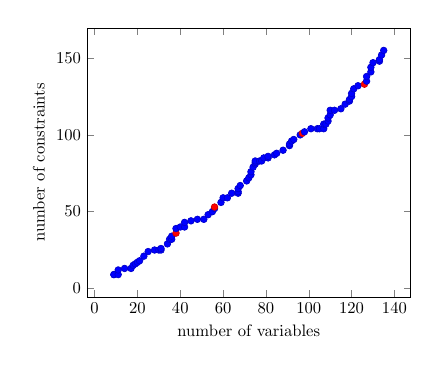
\begin{tikzpicture}[scale=0.6]
\begin{axis}[scatter, point meta=\thisrow{time}, only marks, , xlabel=number of variables,ylabel=number of constraints]

\addplot table[x=x,y=y]  { 
 x y time
 9 9 0.05 
 9 9 0.0 
 11 9 0.0 
 11 12 0.0 
 14 13 0.0 
 17 13 0.0 
 18 15 0.0 
 19 16 0.0 
 20 17 0.0 
 21 18 0.0 
 23 21 0.0 
 25 24 0.0 
 28 25 0.0 
 30 25 0.0 
 31 25 0.0 
 31 26 0.0 
 34 29 0.0 
 35 32 0.0 
 36 32 0.0 
 36 34 0.0 
 38 36 1440.0 
 38 39 0.0 
 40 40 0.0 
 42 40 0.0 
 42 43 0.0 
 45 44 0.0 
 48 45 0.0 
 51 45 0.0 
 53 48 0.0 
 55 50 0.0 
 56 52 0.0 
 56 53 1440.0 
 59 56 0.0 
 60 59 0.0 
 62 59 0.0 
 64 62 0.0 
 67 62 0.0 
 67 63 0.0 
 67 65 0.0 
 68 67 0.0 
 71 70 0.0 
 72 72 0.0 
 73 74 0.0 
 73 76 0.0 
 74 79 0.0 
 75 81 0.0 
 75 82 0.0 
 75 83 0.0 
 77 83 0.0 
 78 83 0.0 
 79 85 0.0 
 81 85 0.0 
 81 86 0.0 
 84 87 0.0 
 85 88 0.0 
 88 90 0.0 
 91 93 0.0 
 91 94 0.0 
 92 96 0.0 
 93 97 0.0 
 96 100 0.0 
 97 101 1440.0 
 98 102 0.0 
 101 104 0.0 
 104 104 0.0 
 105 104 0.0 
 107 104 0.0 
 107 107 0.0 
 108 107 0.0 
 109 109 0.0 
 109 111 0.0 
 110 113 0.0 
 110 116 0.0 
 112 116 0.0 
 115 117 0.0 
 117 120 0.0 
 119 122 0.0 
 119 123 0.0 
 120 125 0.0 
 120 127 0.0 
 121 130 0.0 
 123 132 0.0 
 126 133 1440.0 
 127 135 0.0 
 127 138 0.0 
 129 141 0.0 
 129 144 0.0 
 130 147 0.0 
 133 148 0.0 
 133 149 0.0 
 134 152 0.0 
 135 155 0.0 
};

\end{axis}
\end{tikzpicture}

\\
\\\\
\multicolumn{3}{c}{\ref{storedcolorbar2}}\end{tabular}\end{center}

\newpage

\end{document}